\documentclass[class=jsarticle, crop=false, dvipdfmx, fleqn]{standalone}
%% preamble for Numerical-structure-analysis report

\input{/Users/User/Documents/Project/TeX/preamble/mypreamble}

%% titles
\title{統計的機械学習 レポート}
\author{37-196360 \quad 森田涼介}


%% setting for listings
\newtcbinputlisting[auto counter]{\reportlisting}[3][]{%
	listing file = {#3},
	listing options = {language=python, style=tcblatex, numbers=left, numberstyle=\tiny},
	listing only,
	breakable,
	toprule at break = 0mm,
	bottomrule at break = 0mm,
	left = 6mm,
	sharp corners,
	drop shadow,
	title = Listings \thetcbcounter : \texttt{#2},
	label = #1,
	}



%% title format
\usepackage{titlesec}
\titleformat{\section}{\LARGE}{宿題\thesection}{0zw}{}
\newcommand{\sectionbreak}{\clearpage}
\titleformat{\subsection}{\Large}{\Alph{subsection})}{0zw}{}

\begin{document}
\section{}

二項分布から標本を発生させ,最尤推定量を求める。
また,それを繰り返し,最尤推定量の分布を求める。
標本数を変え,最尤推定量の漸近正規性の確認も行う。


\subsection*{理論}

いま,二項分布では,
\begin{equation}
    q(x;\ \theta) = {}_n\mathrm{C}_x \theta^x (1-\theta)^{n-x}
    \qquad (0 \le \theta \le 1)
\end{equation}
であるから,その対数尤度および対数尤度の\(\theta\)による微分は次のようになる。
\begin{align}
    \log{q(x;\ \theta)}
        & = \log\qty{\frac{n!}{x!(n-x)!} \theta^x (1-\theta)^{n-x}} \\
        & = \log(n!) - \log(x!) - \log((n-x)!) + x\log\theta + (n-x)\log(1-\theta) \\
    \pdv{}{\theta} \qty(q(x;\ \theta))
        & = \frac{x}{\theta} - \frac{n-x}{1-\theta} \\
        & = \frac{x - n\theta}{\theta(1-\theta)} \\
        & = \frac{1}{n} \frac{(x/n) - \theta}{\theta(1-\theta)}
\end{align}
これより,対数尤度を最大にするような\(\theta\),
つまり\(\theta\)の最尤推定量は,
\begin{align}
    \hat{\theta} = \frac{x}{n}
\end{align}
となる。
したがって,
\begin{equation}
    \pdv{}{\theta} \qty(q(x;\ \theta)) = \frac{1}{n} \frac{\hat{\theta} - \theta}{\theta(1-\theta)}
\end{equation}
となる。
また,これを用いると,フィッシャーの情報行列の期待値は次のようになる。
\begin{align}
    \hat{F}(\theta^*)
        & = \frac{1}{N} \sum_{i=1}^{N} \qty(\eval{\pdv{}{\theta} \qty(q(x;\ \theta))}_{\theta = \theta^*})^2 \\
        & = \frac{1}{N} \sum_{i=1}^{N} \qty(\frac{1}{n} \frac{\hat{\theta} - \theta^*}{\theta^* (1-\theta*)})^2
\end{align}



\subsection*{問題設定}

\(\theta^* = 0.3\)であるような二項分布を用い,
標本数\(n = \num{1e1} \mhyphen\mhyphen \num{1e5}\)について,
それぞれ1000回最尤推定量を求めてその分布を求める。
また,正規分布であるかどうかの判別にはシャピロウィルク検定を用いた。
なお,プログラムは\pageref{listing:assignment3}ページのListing \ref{listing:assignment3}に示した。



\subsection*{結果}

表\ref{tab:result}に,各標本数での結果を示す。
なお,\(p\)はシャピロウィルク検定のp値である。
また,各標本数におけるヒストグラムとQQプロットを
図\ref{fig:n10}--\ref{fig:n100000}に示す。

\begin{table}
    \centering
    \caption{各サンプル数における最尤推定量の統計量}
    \begin{tabular}{ccccccc}
        \#Sample & mean & cov & \(F\) & \(1/(nF)\) & \(p\) & Normal Distribution \\
        \num{1e1} & 0.3055 & \num{2.086e-2} & 4.732 & \num{2.113e-2} & \num{3.371e-17} & False \\
        \num{1e2} & 0.3011 & \num{2.200e-3} & 4.988 & \num{2.005e-3} & \num{3.770e-4} & False \\
        \num{1e3} & 0.2998 & \num{2.083e-4} & 4.719 & \num{2.119e-4} & 0.1715 & True \\
        \num{1e4} & 0.3001 & \num{1.891e-5} & 4.285 & \num{2.334e-5} & 0.6772 & True \\
        \num{1e5} & 0.3001 & \num{2.175e-6} & 4.948 & \num{2.021e-6} & 0.4487 & True
    \end{tabular}
    \label{tab:result}
\end{table}


\begin{figure}
	\centering
    \begin{minipage}{0.45\linewidth}
        \begin{figure}[H]
        	   \centering
            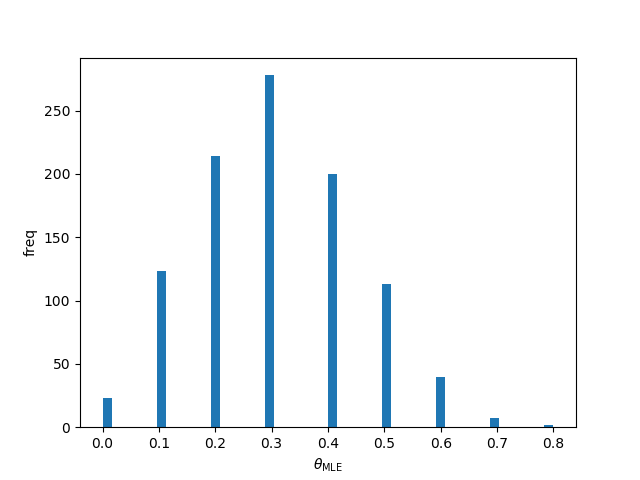
\includegraphics[clip, width=\linewidth]{../figures/hist_n10.png}
            \subcaption{ヒストグラム}
            \label{fig:hist_n10}
        \end{figure}
    \end{minipage}
    \begin{minipage}{0.45\linewidth}
        \begin{figure}[H]
            \centering
            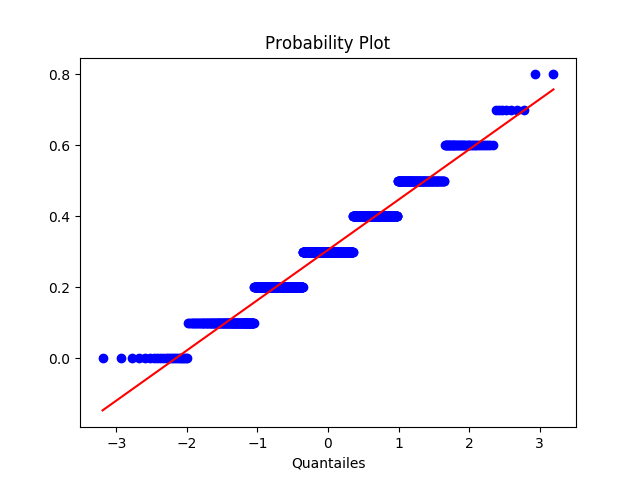
\includegraphics[clip, width=\linewidth]{../figures/qqplot_n10.png}
            \subcaption{QQプロット}
            \label{fig:qqplot_n10}
        \end{figure}
    \end{minipage}
    \caption{標本数10のときの二項分布の最尤推定量のヒストグラムとQQプロット}
    \label{fig:n10}
\end{figure}

\begin{figure}
	\centering
    \begin{minipage}{0.45\linewidth}
        \begin{figure}[H]
            \centering
            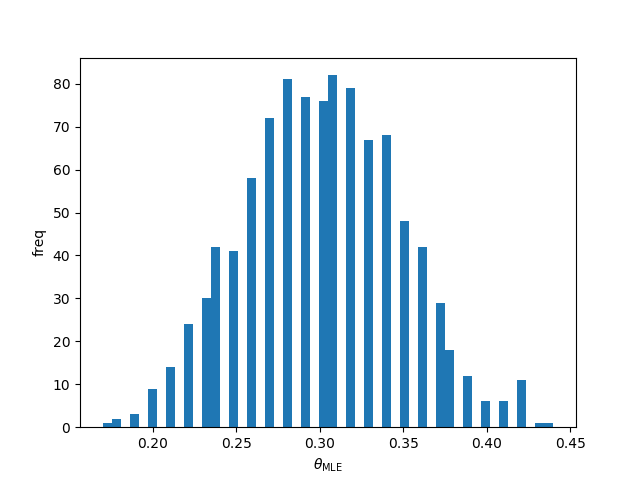
\includegraphics[clip, width=\linewidth]{../figures/hist_n100.png}
            \subcaption{ヒストグラム}
            \label{fig:hist_n100}
        \end{figure}
    \end{minipage}
    \begin{minipage}{0.45\linewidth}
        \begin{figure}[H]
            \centering
            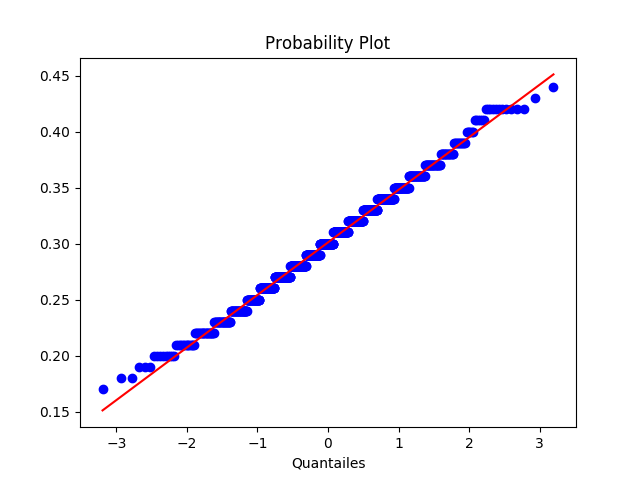
\includegraphics[clip, width=\linewidth]{../figures/qqplot_n100.png}
            \subcaption{QQプロット}
            \label{fig:qqplot_n100}
        \end{figure}
    \end{minipage}
    \caption{標本数100のときの二項分布の最尤推定量のヒストグラムとQQプロット}
    \label{fig:n100}
\end{figure}

\begin{figure}
	\centering
    \begin{minipage}{0.45\linewidth}
        \begin{figure}[H]
            \centering
            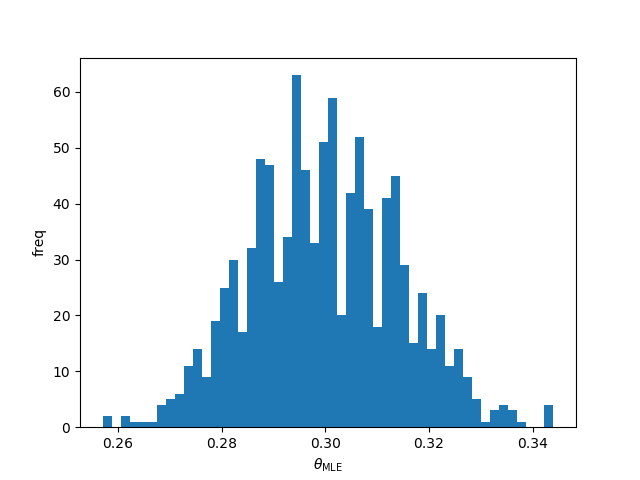
\includegraphics[clip, width=\linewidth]{../figures/hist_n1000.png}
            \subcaption{ヒストグラム}
            \label{fig:hist_n1000}
        \end{figure}
    \end{minipage}
    \begin{minipage}{0.45\linewidth}
        \begin{figure}[H]
            \centering
            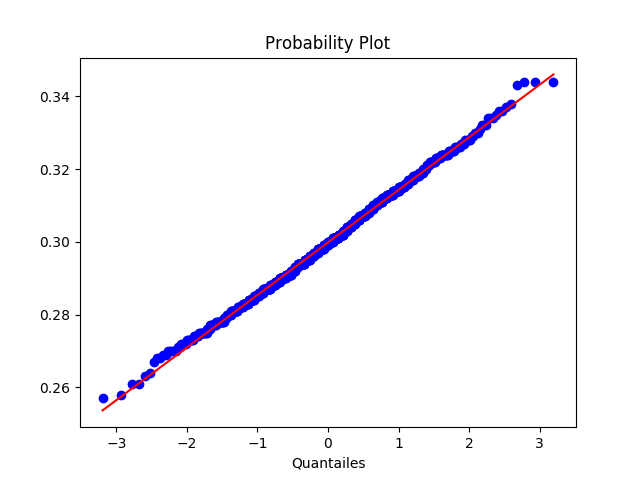
\includegraphics[clip, width=\linewidth]{../figures/qqplot_n1000.png}
            \subcaption{QQプロット}
            \label{fig:qqplot_n1000}
        \end{figure}
    \end{minipage}
    \caption{標本数1000のときの二項分布の最尤推定量のヒストグラムとQQプロット}
    \label{fig:n1000}
\end{figure}

\begin{figure}
	\centering
    \begin{minipage}{0.45\linewidth}
        \begin{figure}[H]
            \centering
            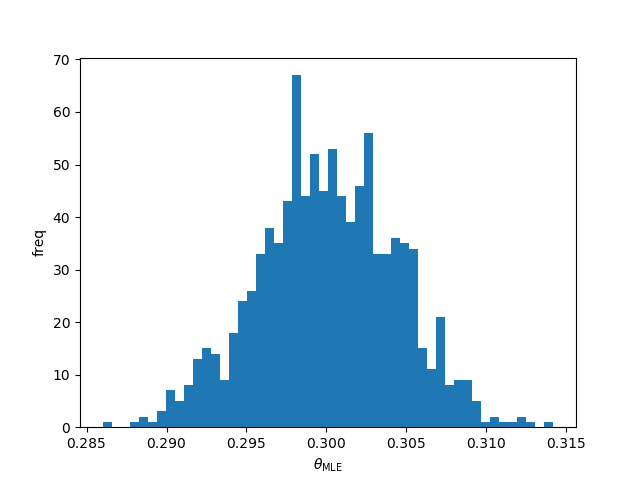
\includegraphics[clip, width=\linewidth]{../figures/hist_n10000.png}
            \subcaption{ヒストグラム}
            \label{fig:hist_n10000}
        \end{figure}
    \end{minipage}
    \begin{minipage}{0.45\linewidth}
        \begin{figure}[H]
            \centering
            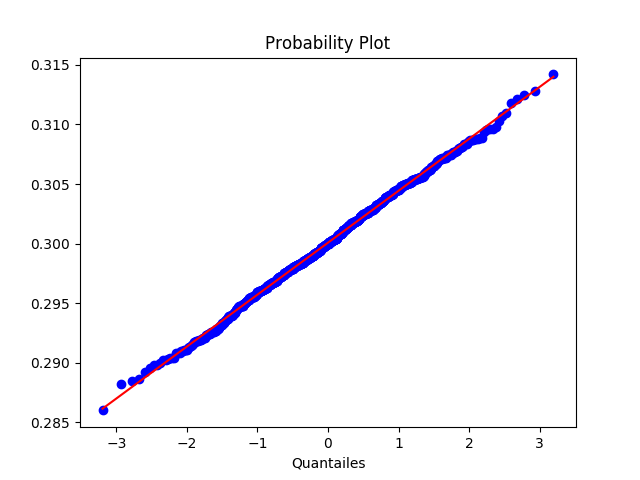
\includegraphics[clip, width=\linewidth]{../figures/qqplot_n10000.png}
            \subcaption{QQプロット}
            \label{fig:qqplot_n10000}
        \end{figure}
    \end{minipage}
    \caption{標本数10000のときの二項分布の最尤推定量のヒストグラムとQQプロット}
    \label{fig:n10000}
\end{figure}

\begin{figure}
	\centering
    \begin{minipage}{0.45\linewidth}
        \begin{figure}[H]
            \centering
            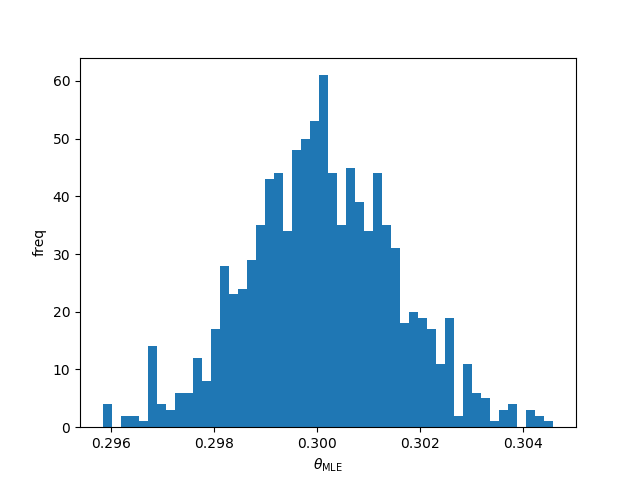
\includegraphics[clip, width=\linewidth]{../figures/hist_n100000.png}
            \subcaption{ヒストグラム}
            \label{fig:hist_n100000}
        \end{figure}
    \end{minipage}
    \begin{minipage}{0.45\linewidth}
        \begin{figure}[H]
            \centering
            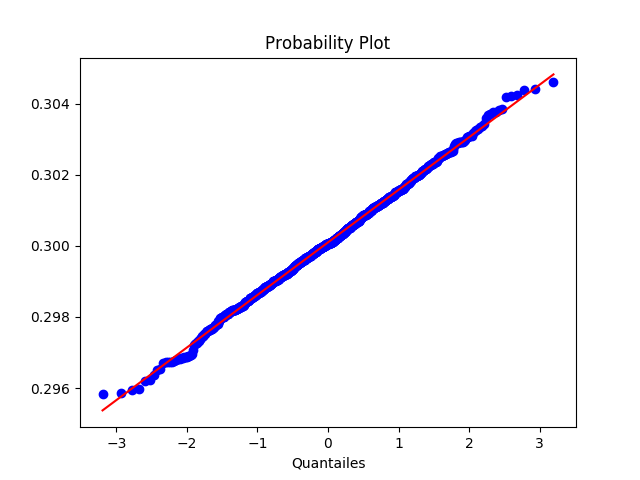
\includegraphics[clip, width=\linewidth]{../figures/qqplot_n100000.png}
            \subcaption{QQプロット}
            \label{fig:qqplot_n100000}
        \end{figure}
    \end{minipage}
    \caption{標本数100000のときの二項分布の最尤推定量のヒストグラムとQQプロット}
    \label{fig:n100000}
\end{figure}



\subsection*{考察}

標本数\(n\)が100以下のときは,
二項分布の最尤推定量の分布は正規分布とはみなされなかった。
しかし,標本数を1000以上にしたところ,
これは正規分布となった。
これらのことから,最尤推定量の漸近正規性が確認された。


\end{document}
